\section[Общесистемная часть]{ОБЩЕСИСТЕМНАЯ ЧАСТЬ}

\subsection{Описание объекта проектирования}

Объектом проектирования является мобильное приложение,
выполняющее учет и представление финансовых данных пользователя.

Ввод данных осуществляется пользователем вручную,
либо с помощью распознавания данных с изображения,
полученного фотокамерой мобильного устройства.

Хранение данных осуществляется средствами мобильной платформы в
виде реляционной базы данных.

Вывод данных сводится к построению различных отчетов об изменении
баланса денежных средств за выбранный период.

\subsection{Постановка задачи проектирования}

Требуется выполнить проектирование автоматизированной системы,
выполненной в виде мобильного приложения и обладающей следующими
функциональными возможностями:
\begin{itemize}
\item ручной ввод финансовых данных с возможностью выбора счета,
  валюты и категории;
\item автоматический ввод финансовых данных с изображения,
  содержащего некоторые числовые данные;
\item хранение финансовых данных в зашифрованном виде;
\item построение графиков изменения баланса денежных средств
  на выбранном счете за выбранный период;
\item построение отчета о расходах пользователя
  за выбранный период с группировкой по категориям.
\end{itemize}

Разработанное приложение должно иметь простой и удобный
пользовательский интерфейс.

\pagebreak
\subsection{Концептуальная модель системы}

В целом, можно выделить следующие сценарии использования приложения:
\begin{itemize}
  \item ввод финансовых данных;
  \item просмотр отчетов на основании накопленных данных.
\end{itemize}

Эти сценарии приведены на рисунке~\ref{fig:use_cases}.

\begin{figure}[h!]
  \centering
  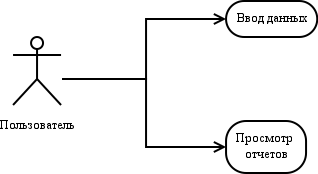
\includegraphics[width=50mm]{pic/use_cases}
  \caption{Диаграмма прецендентов \\ использования приложения}
  \label{fig:use_cases}
\end{figure}

Ввод финансовых данных предполагает ввод значения изменения суммы
денежных средств определенной валюты на определенном счете и категории.
Просмотр отчетов предполагает выборку требуемой информации из базы данных и
её представление в желаемой форме.

Исходя из этого, можно выделить следующие сущности рассматриваемой
предметной области:
\begin{itemize}
\item счета;
\item категории;
\item изменения состояния счета.
\end{itemize}

Эти сущности, а также связи между ними, приведены на рисунке~\ref{fig:entities}.

\begin{figure}[h!]
  \centering
  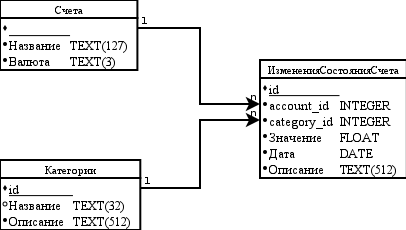
\includegraphics[width=92mm]{pic/entities}
  \caption{Основные сущности предметной области}
  \label{fig:entities}
\end{figure}

Сущность <<Счет>> соответствует, например, платежной карте
и состоит из названия, идентификатора и валюты, в которой производятся расчеты.

Сущность <<Категория>> соответствует некоторой категории доходов или расходов
пользователя, например <<Расходы на еду>>, или <<Заработная плата>>
и состоит из названия, идентификатора и описания.

Сущность <<Изменение состояния счета>> отражает изменение состояния счета
пользователя и включает в себя идентификаторы счета и категории,
значения изменения счета, даты изменения и комментария.